\begin{document}
	%TODO:  La puntuación log(UPSM) y el error de clasificación obtenido en todos los modelos para cada una de las tres clases de modelos.
	% TODO: El mejor modelo seleccionado de cada clase y su justificación de porque es el mejor. Mostrar también el dibujo de la red bayesiana para cada uno de estos tres modelos (incluso para el caso de la red bayesiana naive). Recordar que weka te permite visualizar la red bayesiana del modelo aprendido.
	En aquest apartat, podem veure els valors de la puntuació log(UPSM) i el percentatge d'error de classificació obtinguts en els diferents models de cadascuna de les classes de models. 
	\subsection{Models de la classe 1}
	\begin{enumerate}
		\item \textbf{log(UPSM):} -92608.96126554035 \textbf{Error de classificació:} 48.4167 \%
		\item \textbf{log(UPSM):} -92139.67866809308 \textbf{Error de classificació:} 48.4167 \%
		\item \textbf{log(UPSM):} -92388.27489566772 \textbf{Error de classificació:} 48.4167 \%
		\item \textbf{log(UPSM):} -92227.05224681877 \textbf{Error de classificació:} 48.4484 \%
		\item \textbf{log(UPSM):} -92066.4712487785 \textbf{Error de classificació:} 48.4167 \%
		\item \textbf{log(UPSM):} -92302.15263672064 \textbf{Error de classificació:} 48.4167 \%
		\item \textbf{log(UPSM):} -92180.71383973274 \textbf{Error de classificació:} 48.4167 \%
		\item \textbf{log(UPSM):} -92586.42609497187 \textbf{Error de classificació:} 48.4167 \%
		\item \textbf{log(UPSM):} -92245.67223271335 \textbf{Error de classificació:} 48.4167 \%
		\item \textbf{log(UPSM):} -93188.71009303001 \textbf{Error de classificació:} 48.4167 \%
	\end{enumerate}
	\vspace{0.5cm}
	Per a poder seleccionar el millor model dels anteriors, ens hem de fixar sobretot en quin d'ells ens classifica correctament un major nombre d'instàncies i, per tant, vaga la redundància, quin model té el menor percentatge d'error de classificació.\\
	Com podem observar, tots els models tenen el mateix percentatge d'error excepte un, el qual podem descartar directament, ja que és més alt que la resta. Entre els altres models, no ens sorpèn que el percentatge no variï, ja que observant les dades que se'ns donaven inicialment i després de separar-les en els conjunts d'aprenentatge i testing, veiem una tendència d'un 50\% de casos en els quals el valor del overall\_satisfaction és de 4.5.\\\\
	Per tant, veient totes les dades, podem arribar a la conclusió que ens podriem trobar en una situació d'"empat". Una manera de resoldre'l, i la que utilitzarem, serà comparar els valros del log(UPSM) de cada model.\\
	Per concloure, considerarem que, el millor model d'entre els que tenen el mateix i millor percentatge en aquesta classe, serà aquell que tingui un UPSM socre més elevat, es a dir, el model que el seu log(UPSM) sigui més baix. Per tant, considerarem com a millor model de la classe 1, el classificat amb el nombre 5, del qual es pot observar la seva representació gràfica a la Figura \ref{fig:model1}.
	\begin{figure}[H]
		\centering
		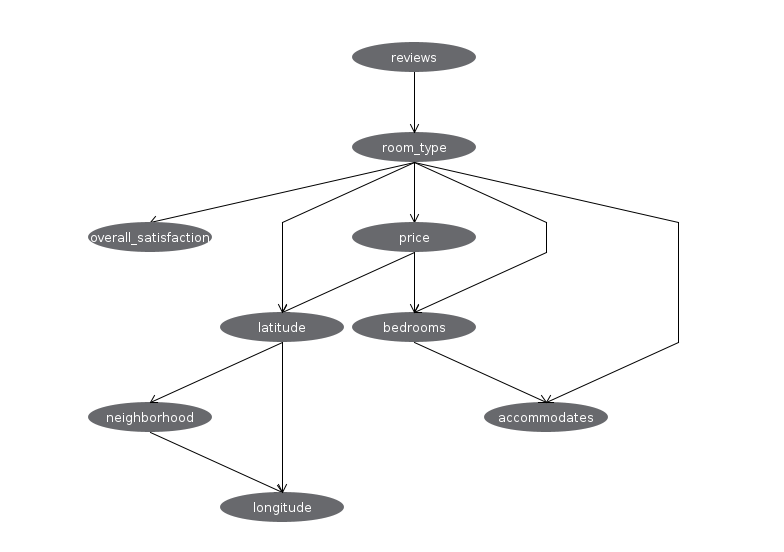
\includegraphics[width=12cm]{imgs/modelclasse1.png}
		\caption{Millor model de la classe 1}
		\label{fig:model1}
	\end{figure}
	\vspace{0.5cm}
	
	\subsection{Model de la classe 2}
	\begin{enumerate}
		\item \textbf{log(UPSM):} -117515.15847723951 \textbf{Error de classificació:} 48.4484 \%
	\end{enumerate}
	\vspace{0.5cm}
	En el cas de la segona classe, només hi trobem un model possible, per tant, serà aquest ek qual considerarem com a millor. El fet que només n'hi hagi un de possible és degut a que aquest model és el corresponent a la xarxa bayesiana naive, tenint com a variable de classe overall\_satisfaction, el qual és un model únic.\\
	A la figura \ref{fig:model2} es pot veure la representació gràfica d'aquest model.
	\vspace{0.3cm}
	\begin{figure}[H]
		\centering
		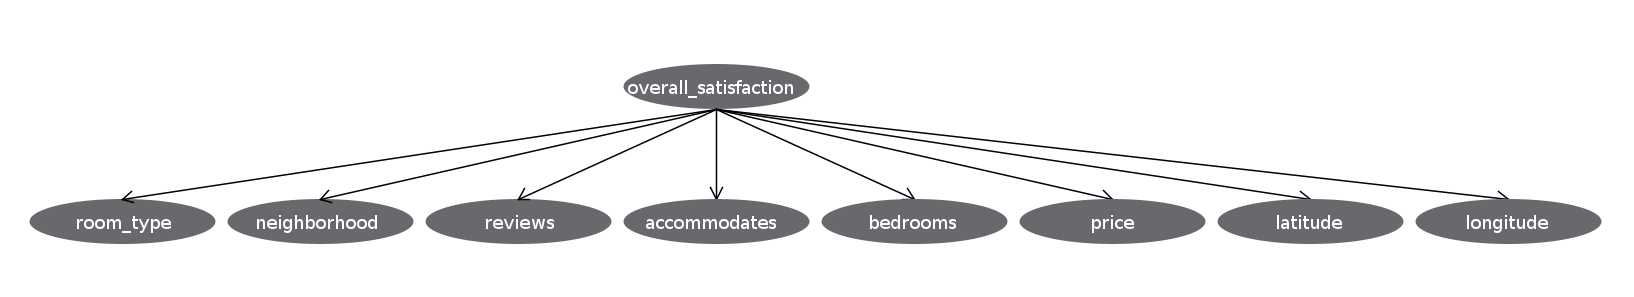
\includegraphics[width=15cm]{imgs/model2.png}
		\caption{Millor model de la classe 2}
		\label{fig:model2}
	\end{figure}
	\vspace{0.5cm}
	\subsection{Models de la classe 3}
	\begin{enumerate}
		\item \textbf{log(UPSM):} -96800.35169816265 \textbf{Error de classificació:} 48.3534 \%
		\item \textbf{log(UPSM):} -95829.88423245584 \textbf{Error de classificació:} 48.86 \%
		\item \textbf{log(UPSM):} -95565.62218051209 \textbf{Error de classificació:} 48.8284 \%
		\item \textbf{log(UPSM):} -95859.94046082163 \textbf{Error de classificació:} 48.4167 \%
		\item \textbf{log(UPSM):} -97231.01625115846 \textbf{Error de classificació:} 48.7334 \%
		\item \textbf{log(UPSM):} -96894.65682950999 \textbf{Error de classificació:} 48.3217 \%
		\item \textbf{log(UPSM):} -95822.6410503832 \textbf{Error de classificació:} 48.67 \%
		\item \textbf{log(UPSM):} -97094.31982431604 \textbf{Error de classificació:} 48.1951 \%
		\item \textbf{log(UPSM):} -95604.5241813889 \textbf{Error de classificació:} 48.575 \%
		\item \textbf{log(UPSM):} -96108.4925816474 \textbf{Error de classificació:} 48.3534 \%
	\end{enumerate}
	\vspace{0.5cm}
	Per tal de poder escollir el millor model d'aquesta classe, s'ha fet de la mateixa manera que en la classe 1. Tot i això, en aquest cas sí que hem pogut veure més diversitat de percentatges d'error en els diferents models. I, per aquest motiu, no ha estat necessàri comparar les valors del UPSM.\\\\
	Els percentatges son bastant semblant entre si, ja que el fet d'enceratr algunes variables més que un altre model, no implica un gran canvi en el percentateg d'encerts, degut a la gran quantitat d'instàncies que tenim en el test. Malgrat tot, hi ha hagut un model que ha encertat algunes instàncies més que la resta. Per tant, considerem com a millor model de la classe 3, el classificat amb el nombre 8, del qual es pot observar la seva representació gràfica a la Figura \ref{fig:model3}.
	\begin{figure}[H]
		\centering
		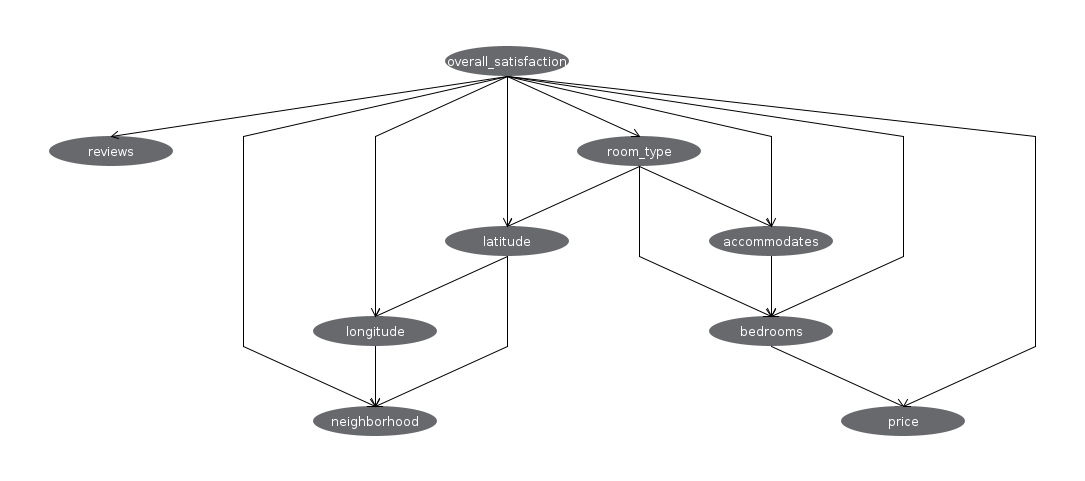
\includegraphics[width=15cm]{imgs/modelclasse3.png}
		\caption{Millor model de la classe 3}
		\label{fig:model3}
	\end{figure}
\end{document}